%%
%% Automatically generated file from DocOnce source
%% (https://github.com/hplgit/doconce/)
%%
%%


%-------------------- begin preamble ----------------------

\documentclass[%
oneside,                 % oneside: electronic viewing, twoside: printing
final,                   % draft: marks overfull hboxes, figures with paths
10pt]{article}

\listfiles               %  print all files needed to compile this document
\usepackage{url}			% needed for citing
\usepackage{relsize,makeidx,color,setspace,amsmath,amsfonts,amssymb}
\usepackage[table]{xcolor}
\usepackage{bm,ltablex,microtype}
\newcommand{\R}{\mathbb{R}}

\usepackage[pdftex]{graphicx}

\usepackage{fancyvrb} % packages needed for verbatim environments

\usepackage[T1]{fontenc}
%\usepackage[latin1]{inputenc}
\usepackage{ucs}
\usepackage[utf8x]{inputenc}

\usepackage{lmodern}         % Latin Modern fonts derived from Computer Modern

% Hyperlinks in PDF:
\definecolor{linkcolor}{rgb}{0,0,0.4}
\usepackage{hyperref}
\hypersetup{
    breaklinks=true,
    colorlinks=true,
    linkcolor=linkcolor,
    urlcolor=linkcolor,
    citecolor=black,
    filecolor=black,
    %filecolor=blue,
    pdfmenubar=true,
    pdftoolbar=true,
    bookmarksdepth=3   % Uncomment (and tweak) for PDF bookmarks with more levels than the TOC
    }
%\hyperbaseurl{}   % hyperlinks are relative to this root

\setcounter{tocdepth}{2}  % levels in table of contents

% --- fancyhdr package for fancy headers ---
\usepackage{fancyhdr}
\fancyhf{} % sets both header and footer to nothing
\renewcommand{\headrulewidth}{0pt}
\fancyfoot[LE,RO]{\thepage}
% Ensure copyright on titlepage (article style) and chapter pages (book style)
\fancypagestyle{plain}{
  \fancyhf{}
  %\fancyfoot[C]{{\footnotesize \copyright\ 1999-2020, "Computational Physics I FYS3150/FYS4150":"http://www.uio.no/studier/emner/matnat/fys/FYS3150/index-eng.html". Released under CC Attribution-NonCommercial 4.0 license}}
%  \renewcommand{\footrulewidth}{0mm}
  \renewcommand{\headrulewidth}{0mm}
}
% Ensure copyright on titlepages with \thispagestyle{empty}
\fancypagestyle{empty}{
  \fancyhf{}
  %\fancyfoot[C]{{\footnotesize \copyright\ 1999-2020, "Computational Physics I FYS3150/FYS4150":"http://www.uio.no/studier/emner/matnat/fys/FYS3150/index-eng.html". Released under CC Attribution-NonCommercial 4.0 license}}
  \renewcommand{\footrulewidth}{0mm}
  \renewcommand{\headrulewidth}{0mm}
}

\pagestyle{fancy}


% prevent orhpans and widows
\clubpenalty = 10000
\widowpenalty = 10000

% --- end of standard preamble for documents ---


% insert custom LaTeX commands...

\raggedbottom
\makeindex
\usepackage[totoc]{idxlayout}   % for index in the toc
\usepackage[nottoc]{tocbibind}  % for references/bibliography in the toc

\usepackage{booktabs}				% for citing
\usepackage{float}					% for placing figures
%-------------------- end preamble ----------------------

\begin{document}

% matching end for #ifdef PREAMBLE

\newcommand{\exercisesection}[1]{\subsection*{#1}}


% ------------------- main content ----------------------



% ----------------- title -------------------------
%
%\thispagestyle{empty}
%
%\begin{center}
%{\LARGE\bf
%\begin{spacing}{1.25}
%Project 1
%\end{spacing}
%}
%\end{center}
%
%% ----------------- author(s) -------------------------
%
%\begin{center}
%{\bf \href{{http://www.uio.no/studier/emner/matnat/fys/FYS3150/index-eng.html}}{Computational Physics I FYS3150/FYS4150}}
%\end{center}
%
%    \begin{center}
%% List of all institutions:
%\centerline{{\small Department of Physics, University of Oslo, Norway}}
%\end{center}
%    
%% ----------------- end author(s) -------------------------
%
%% --- begin date ---
%\begin{center}
%September, 2020
%\end{center}
%% --- end date ---
%
%\vspace{1cm}



%\subsection*{Abstract}
%\subsection*{Introduction}
%\subsection*{Method}
\section*{Abstract}
\section*{Introduction}
\section*{Method}
\paragraph{Approximation of the second derivative}
Given the one-dimensional Poisson equation with Dirichlet boundary conditions
\begin{equation*}
-u''(x) = f(x), \hspace{0.5cm} x\in(0,1), \hspace{0.5cm} u(0) = u(1) = 0.
\end{equation*}
we approximate the second derivative of $u$ with
\begin{equation}\label{eqn:2ndDeriv}
   -\frac{v_{i+1}+v_{i-1}-2v_i}{h^2} = f_i  \hspace{0.5cm} \mathrm{for} \hspace{0.1cm} i=1,\dots, n-1,
\end{equation}
where $f_i=f(x_i)$ and the discretized approximation to $u$ is $v_i$ with grid points $x_i = ih$ in the interval from $x_0$ to $x_{n+1}=1$.
Further, the step length, h,  is defined as $h=1/(n+1)$ and the boundary conditions set $v_0 = v_{n+1}=0$. \\
For numerical computation, (\ref{eqn:2ndDeriv}) must be written as a linear set of equations of the form
\begin{equation*}
   \mathbf{A}\mathbf{v} = \tilde{\mathbf{g}},
\end{equation*}
where $\mathbf{A}$ is an $n\times n$  tridiagonal matrix.\\
The set of equation for $h^2f_i$ is given by
\begin{equation*}
   -v_{i+1}-v_{i-1}+2v_i = h^2f_i  \hspace{0.5cm} 
\end{equation*}
Rearranging the equation gives
\begin{equation}
  -v_{i-1}+2v_i - v_{i+1}= h^2f_i  \hspace{0.5cm} 
\end{equation}
Determining the equations for the boundary condition, $i=1$ holds 
\begin{equation}
\begin{aligned}
  -v_{0}+2v_1 - v_{2}&= h^2f_1  \hspace{0.5cm} \\
  0 + 2v_1 - v_{2}&= h^2f_1  \hspace{0.5cm} 
\end{aligned}
\end{equation}

since $v_0=0$. Given $v_{n+1}=0$, similarly for $i=n$ applies
\begin{equation}
\begin{aligned}
  -v_{n-1}+2vn - v_{n+1}&= h^2f_n  \hspace{0.5cm} \\
 -v_{n-1}+ 2v_n - 0&= h^2f_n  \hspace{0.5cm} 
\end{aligned}
\end{equation}
A combination of the above equations results in 
\begin{equation}
\begin{aligned}
  2v_1 - v_{2}&= h^2f_1 & = \tilde{g_1}  \hspace{0.5cm} \\
  ...\\
  -v_{i-1}+2v_i - v_{i+1}&= h^2f_i &= \tilde{g_i}  \hspace{0.5cm} \\
  ...\\
 -v_{n-1}+ 2v_n &= h^2f_n &= \tilde{g_n}  \hspace{0.5cm} 
\end{aligned}
\end{equation}
Thus, there are $n-1$ equations that must be computed ($i \in [1,n-1])$.
The set of equations can be rewritten in matrix-form, there $ \mathbf{A} \in \R^{n \times n} $ and $ \mathbf{v}, \mathbf{g} \in \R^{n}$
\[
     \begin{bmatrix}
                           2& -1 & 0 &\dots   & \dots &\dots \\
                           -1 & 2 & -1 &\dots &\dots &\dots \\
                           & -1 & 2 & -1 & \dots & \dots \\
                           & \dots   & \dots &\dots   &\dots & \dots \\
                           &   &  &-1  &2& -1 \\
                           &    &  &   &-1 & 2 \\
                      \end{bmatrix}\begin{bmatrix}
                           v_1\\
                           v_2\\
                           \dots \\
                          \dots  \\
                          \dots \\
                           v_n\\
                      \end{bmatrix}
  =\begin{bmatrix}
                           g_1\\
                          g_2\\
                           \dots \\
                           \dots \\
                          \dots \\
                           g_n\\
                      \end{bmatrix}.
\]
For simplicity, $v_i$ is from now on written as $u_i$.
Furhter, the vectors $ \mathbf{a}, \mathbf{b}, \mathbf{c}$ are defined as the matrix-elements, there $ \mathbf{b}$ is placed along the diagonal, $\mathbf{a}$ is the lower diagonal and $\mathbf{c}$ is the upper diagonal. $g_i$ stands for $h^2f_i$, the solution for each equation (called source term) \\
\[
    \mathbf{A} = \begin{bmatrix}
                           b_1& c_1 & 0 &\dots   & \dots &\dots \\
                           a_1 & b_2 & c_2 &\dots &\dots &\dots \\
                           & a_2 & b_3 & c_3 & \dots & \dots \\
                           & \dots   & \dots &\dots   &\dots & \dots \\
                           &   &  &a_{n-2}  &b_{n-1}& c_{n-1} \\
                           &    &  &   &a_{n-1} & b_n \\
                      \end{bmatrix}\begin{bmatrix}
                           u_1\\
                           u_2\\
                           \dots \\
                          \dots  \\
                          \dots \\
                           u_n\\
                      \end{bmatrix}
  =\begin{bmatrix}
                           g_1\\
                           g_2\\
                           \dots \\
                           \dots \\
                          \dots \\
                           g_n\\
                      \end{bmatrix}.
\]
In our project, the source term is predefined to be $f(x) = 100e^{-10x}$. Given the above defined boundary conditions, this differential equation has a closed-form solution given by $u(x) = 1 - (1-e^{-10})x -e^{-10x}$. Hereafter, the function values for $u(x)$ are called $\mathbf{exact}$.
 
This linear set of equations can be solved by for example using the Thomas algorithm or the LU decomposition.
\paragraph{Thomas Algorithm}
The Thomas algorithm can be divided into two steps: a forward substitution and a backward substitution \cite{ThomasAlgo}.\\
In the forward substitution, the lower-diagonal elements are eliminated. Starting from the top, this is done by summing two successive appropriately scaled rows in the matrix. The mathematical expression for the new matrix elements is given as
\begin{equation}
\begin{aligned}
\tilde{b}_i &= b_i - a_{j-1} \cdot c_{i-1}/ \tilde{b}_{i-1}  \hspace{0.5cm} \mathrm{for} \hspace{0.1cm} i=2,..., n-1 \\
\tilde{g}_i &= g_i - a_{j-1} \cdot \tilde{g}_{i-1} / \tilde{b}_{i-1}  \hspace{0.5cm} \mathrm{for} \hspace{0.1cm} i=2,..., n-1
\end{aligned}
\end{equation}
The first row remains unchanged. \\
The backward substitution starts at the last row of the matrix. Here, the expression for $u_{n-1}$ becomes immediately clear
\begin{equation}
\begin{aligned}
\tilde{b}_{n-1} u_{n-1} &= \tilde{g}_{n-1} \\
u_{n-1} &= \tilde{g}_{n-1} / \tilde{b}_{n-1}
\end{aligned}
\end{equation}
Going up row for row, $u_i$ can be expressed as
\begin{equation}
u_i = ( \tilde{g_i}-c_i u_{i+1} )/ \tilde{b_i} \hspace{0.5cm} \mathrm{for} \hspace{0.1cm} i=n-2,...,1 
\end{equation}

\subparagraph{Special Case}
For our computation, we set identical matrix elements along the diagonal and identical (but different) values for the non-diagonal elements. More specific, we set $b_j = 2$ and $a_j = c_j = -1$. Thus the Thomas algorithm can be specialized to our specific case. It can be shown that the elements along the diagonal can be precalculated with
\begin{equation}
\tilde{b_i} = \frac{i+1}{i} \hspace{0.5cm} \mathrm{for} \hspace{0.1cm} i=1,...,n-1 
\end{equation}
That means that $\mathbf{\tilde{b}}$ no longer needs to be computed in the forward loop. \\
The forward loop is therefore given by
\begin{equation}
\tilde{g}_i = g_i - a_{j-1} \cdot \tilde{g}_{i-1} / \tilde{b}_{pre, i-1}  \hspace{0.5cm} \mathrm{for} \hspace{0.1cm} i=2,..., n-1 \\
\end{equation}
there $\tilde{b}_{pre}$ stands for the precalculation.
Similarly, the backward loop is now also computed with the precalculated $\mathbf{\tilde{b}}$
\begin{equation}
u_i = ( \tilde{g_i}-c_i u_{i+1} )/ \tilde{b}_{pre,i} \hspace{0.5cm} \mathrm{for} \hspace{0.1cm} i=n-2,...,1 
\end{equation}
The tables below (Table \ref{tbl: G_FLOPS} and Table \ref{tbl: S_FLOPS}) show what effect this precalculation has on the number of FLOPs in the forward and backward substitution.

\begin{table}[H]
\caption{FLOPS for general algorithm}
\centering
	\begin{tabular}{r r r r}
		\toprule
		FLOPs   & Forward & Backward & Total \\ [0.5ex]
		\midrule
		$\mathbf{b}$ & $3 (n-2)$       & -        & -    \\
		$\mathbf{g}$ & $3 (n-2)$       & -       & -    \\
        	$\mathbf{u}$ & -      & $3 (n-2)$         & -     \\
        	Total        & $6 (n-2)$       & $3 (n-2)$        &  $9 (n-2)$      \\ [1ex]
		\bottomrule
	\end{tabular}
	\label{tbl: G_FLOPS}
\end{table}	

\begin{table}[H]
\caption{FLOPS for special algorithm}
\centering
	\begin{tabular}{r r r r}
		\toprule
		FLOPs   & Forward & Backward & Total \\ [0.5ex]
		\midrule
		$\mathbf{g}$ & $2 (n-2)$       & -        & -    \\
        	$\mathbf{u}$ & -       & $2 (n-2)$        & -     \\
        	Total        & $2 (n-2)$       & $2 (n-2)$  & $4 (n-2)$      \\ [1ex]
		\bottomrule
	\end{tabular}
	\label{tbl: S_FLOPS}
\end{table}	

For the special algorithm, the $2(n-1)$ FLOPs for the precalculated $\mathbf{b}$ must be taken into consideration. If n is a large number, the following approximation applies: $n-2 \approx n-1 \approx n$. Thus, comparing the two algorithms, the number of FLOPs are reduced from $9n$ (general) to $6n$ (special).

\paragraph{LU decomposition}
Another way to solve the set of linear equations is the LU decomposition  \cite{LUdecomp}.
This method factorizes the given square $\mathbf{A}$ matrix into two triangular matrices, one lower triangular matrix, $ \mathbf{L}$, and one upper triangular matrix, $\mathbf{U}$.
The original matrix $\mathbf{A}$ is then given by their matrix-product, i.e. $ \mathbf{A}= \mathbf{L} \mathbf{U}$.
The Gauss Elimination Method is used on $\mathbf{A}$ to form $\mathbf{U}$.
The diagonal elements of $\mathbf{L}$ er set to one. For a $3 \times 3$ matrix $\mathbf{A}$, the LU decomposition would look like
\[
     \begin{bmatrix}
                           a_{11}	& a_{12} & a_{13} \\
                           a_{21} & a_{22} & a_{23}  \\
                           a_{31} & a_{32} & a_{33}  \\
                      \end{bmatrix}
  =\begin{bmatrix}
                           1		& 0 & 0 \\
                           l_{21} & 1 & 0  \\
                           l_{31} & l_{32} & 1  \\
                      \end{bmatrix}
   \begin{bmatrix}
                           u_{11}& u_{12} & u_{13} \\
                           0 		& u_{22} & u_{23}  \\
                           0 		& 0 & u_{33}  \\
                      \end{bmatrix}
\]
The LU decomposition allows to rewrite the equation $\mathbf{Ax} = \mathbf{g}$ into two systems
\begin{equation}
\begin{aligned}
\mathbf{Ly} &= \mathbf{g} \\
\mathbf{Ux} &= \mathbf{y}
\end{aligned}
\end{equation}
Forward substitution can be used to solve the system $\mathbf{Ly} = \mathbf{g}$ and backward substitution can be used to solve $\mathbf{Ux} = \mathbf{y}$.
\paragraph{General Algorithm}
%http://folk.ntnu.no/leifh/teaching/tkt4140/._main040.html
Given below are pseudocodes for the Thomas algorithm and the LU decomposition.
\subparagraph{Thomas Algorithm}
\begin{enumerate}
\item Setting the input variables (x0, xn, a, b, c, n) \\
	x0 and xn confine the interval (here from 0 to 1). \\
	n stands for the number of integration points. \\
	In our case, the elements along the tridiagonal are constant, e.g. $a_i=a$, $b_i=b, c_i=c$ for all i. 
	
\item Initialization: Defining the step size h. \\
	Allocation of memory for $ \mathbf{a}, \mathbf{b}, \mathbf{c}, \mathbf{g}, \mathbf{u}, \mathbf{exact}$\\
	 $ \mathbf{a}, \mathbf{b}, \mathbf{c}, \mathbf{g}$ have length n, whereas $\mathbf{u}, \mathbf{exact}$ have length n+1\\
	for (i=1, n-1): \\
		 general: set $a_i=a$, $b_i=b, c_i=c$ \\
		 special: set $a_i=a, c_i=c, b_i=(i+1)/i$ \\
		 compute $\mathbf{exact}$  

\item Thomas algorithm with forward substitution\\
	 for (2=1, n-1):\\
	general case: update $\mathbf{b}, \mathbf{g}$ \\
	special case: update $\mathbf{g}$

\item Thomas algorithm with backward substitution \\
	 while (i=n-2, 1):\\ 
	 compute $\mathbf{u}$ (general / special case)

\item Testing analytic solution: compute relative error $  \epsilon =  \left\lvert \frac{u_i-exact_i}{exact_i} \right\rvert$ 

\item Measure average CPU time for the different algorithms

\item Write results to file and if applicable plot them
\end{enumerate}

\subparagraph{LU decomposition}
Using armadillo with its build-in functions
\begin{enumerate}
\item Initialize Setting the input variables (x0, xn, a, b, c, n) \\
	x0 and xn confine the interval (here from 0 to 1). \\
	n stands for the number of integration points. \\
	In our case, the elements along the tridiagonal are constant, e.g. $a_i=a$, $b_i=b, c_i=c$ for all i. 

\item Setting up matrix $\mathbf{A}^{n-1 \times n-1}$ using built-in function (i.e. mat A = zeros<mat>(n-1,n-1)\\
	 for(1, n-2): \\
	 Fill up matrix \\
	 First and last row must be set separately
		
\item Compute $\mathbf{L}$ and $\mathbf{U}$ (built-in function)

\item Compute $\mathbf{y}$ in $\mathbf{Ly}=\mathbf{g}$ using forward substitution (built-in function)

\item Compute $\mathbf{x}$ in $\mathbf{Ux}=\mathbf{y}$ using backward substitution (built-in function)\\
		$\mathbf{x}$ is the solution-vector $\mathbf{u}$ 

\item Measure average CPU time		
\end{enumerate}
To ensure that all 3 algorithms have been implemented correctly, the computed solution for the general and special Thomas algorithm and LU method, for n=10, are given below. As comparison serves the given correct solution.

\section*{Results}
First, the results for computing the general Thomas algorithm are given for the matrices of the size $10 \times 10$, $100 \times 100$, $1000 \times 1000$ (corresponding to $n=10$, $n=100$ and $n=1000$), in the interval $x \in (0,1)$. The computed solution is graphed together with the exact solution.

\begin{figure}[H]
\begin{center}
\graphicspath{ {ComputedvsExact/} }
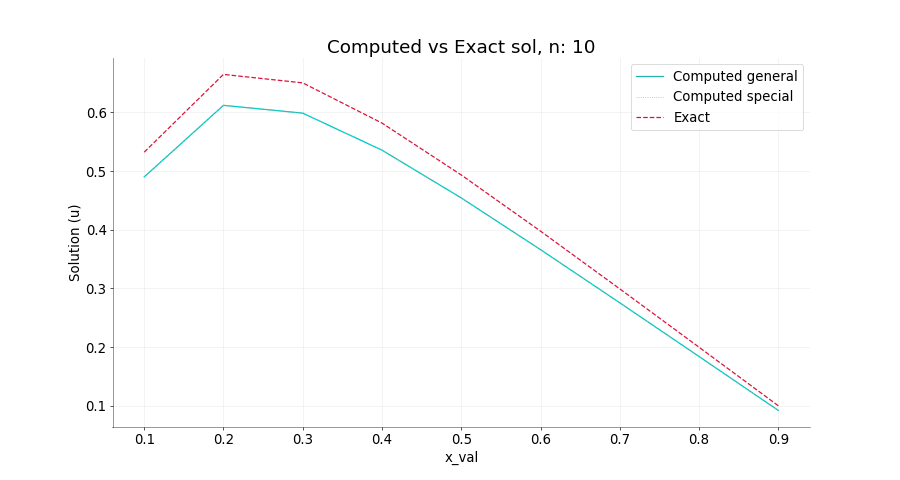
\includegraphics[width=10cm]{ComputedvsExact_sol_n10.png}
\caption{general Thomas algorithm graphed with exact solution (n=10)}
\end{center}
\end{figure}

\begin{figure}[H]
\begin{center}
\graphicspath{ {ComputedvsExact/} }
\includegraphics[width=10cm]{ComputedvsExact_sol_n100.0.png}
\caption{general Thomas algorithm graphed with exact solution (n=100)}
\end{center}
\end{figure}

\begin{figure}[H]
\begin{center}
\graphicspath{ {ComputedvsExact/} }
\includegraphics[width=10cm]{ComputedvsExact_sol_n1000.0.png}
\caption{general Thomas algorithm graphed with exact solution (n=1000)}
\end{center}
\end{figure}

Next, the table below (Table \ref{CPUtime}) shows the CPU time for the general and special Thomas algorithm for matrices up to $n=10^6$. As the CPU time measurement can be random, the average time of 40 repetitions was taken.
\begin{table}[H]
\caption{CPU time for all 3 algorithms}
\centering
\begin{tabular}{rrrr}
\toprule
    n & General time[s] & Special time[s] & LU time[s] \\
\midrule
    10 &    2.250E-06 &    2.425E-06 &  8.593E-05 \\
   100 &    8.250E-06 &    7.250E-06 &  1.251E-03 \\
   1000 &    7.240E-05 &    6.593E-05 &  1.270E-01 \\
  10000 &    9.013E-04 &    7.289E-04 &  8.675E+01 \\
  100000 &    8.585E-03 &    6.494E-03 &     NAN \\
 1000000 &    8.745E-02 &    6.564E-02 &     NAN \\
 10000000 &    9.784E-01 &    8.487E-01 &     NAN \\
\bottomrule
\end{tabular}
\label{CPUtime}
\end{table}
As expected, the special Thomas algorithm is the most rapid and LU decomposition the slowest. Since the LU method makes use of a whole matrix (instead of only allocating the tridiagonal using arrays), the memory space is to little if $n>10^4$. That is, we only get results for $n<10^5$.
For every step, the LU time increases notably.\\
Even though the FLOPS for the special algorithm are reduced from $9n$ (general algorithm) to $6n$, other factors such as fetching variables must be considered. Moreover, the measured time is affected by the PC's granularity, temperature of the processor, number of chores the CPU is processing and so forth. This might explain why the time difference between the general and special algorithm is less than expected.

To check the accuracy of the general Thomas algorithm, the relative error, $  \epsilon =  \left\lvert \frac{u_i-exact_i}{exact_i} \right\rvert$, in the data set $i=1,...n-1$, is given in Table \ref{LogError}. The max error-value for each step was taken.
\begin{table}[H]
\caption{logarithmic error for the general Thomas algorithm}
\centering
\begin{tabular}{rr}
\toprule
    n &  LogErr \\
\midrule
  10.0 & -1.100582 \\
  100.0 & -3.079398 \\
 1000.0 & -5.079183 \\
 10000.0 & -7.079199 \\
\bottomrule
\end{tabular}
\label{LogError}
\end{table}
The relative error decreases with increasing $n$ as expected. Further, the error declines by a factor of $10^2$ for each each step. In general, the computed solution is quite precise. In comparison, single machine precision is in order of $10^{-7}$.



\section*{Conclusion}

%https://www.geeksforgeeks.org/l-u-decomposition-system-linear-equations/
%http://www.math4all.in/public_html/linear%20algebra/chapter2.7.html







\bibliography{citation}
\bibliographystyle{ieeetr}

% ------------------- end of main content ---------------

\end{document}

